\documentclass[12pt,a4paper]{article}

% Language setting
\usepackage[portuguese]{babel}
%\addto\captionsportuguese{\newcommand{\andname}{e}}

% Set page size and margins
\usepackage[a4paper,top=2cm,bottom=2cm,left=2.5cm,right=2.5cm,marginparwidth=1.75cm]{geometry}


\usepackage{amsmath}
\usepackage{graphicx}
\usepackage[colorlinks=true, allcolors=blue]{hyperref}
\usepackage{hyperref}
\usepackage{orcidlink}
\usepackage[title]{appendix}
\usepackage{mathrsfs}
\usepackage{amsfonts}
\usepackage{booktabs} % For \toprule, \midrule, \botrule
\usepackage{caption}  % For \caption
\usepackage{threeparttable} % For table footnotes
\usepackage{listings}
\usepackage{enumitem}
\usepackage{chngcntr}
\usepackage{booktabs}
\usepackage{lipsum}
\usepackage{subcaption}
\usepackage{authblk}
\usepackage[T1]{fontenc}    % Font encoding
\usepackage{csquotes}       % Include csquotes
\usepackage{diagbox}


% Customize line spacing
\usepackage{setspace}
\onehalfspacing % 1.5 line spacing

% Redefine section and subsection numbering format
\usepackage{titlesec}
\titleformat{\section} % Redefine section numbering format
  {\normalfont\Large\bfseries}{\thesection.}{1em}{}

% Change the position of the table caption above the table
\usepackage{float}   % for customizing caption position
\usepackage{caption} % for customizing caption format
\captionsetup[table]{position=top} % caption position for tables

% Define the unnumbered list
\makeatletter
\newenvironment{unlist}{%
  \begin{list}{}{%
    \setlength{\labelwidth}{0pt}%
    \setlength{\labelsep}{0pt}%
    \setlength{\leftmargin}{2em}%
    \setlength{\itemindent}{-2em}%
    \setlength{\topsep}{\medskipamount}%
    \setlength{\itemsep}{3pt}%
  }%
}{%
  \end{list}%
}
\makeatother

% Suppress the warning about \@parboxrestore
\pdfsuppresswarningpagegroup=1

%-------------------------------------------
% Paper Head
%-------------------------------------------
\title{PTC3314 - Ondas e Linhas}
\author{1º Exercício de Simulação Computacional}

\affil{Guilherme Fortunato Miranda, Nº USP: 13683786}
\affil{João Pedro Dionizio Calazans, Nº USP: 13673086}
\affil{Thomas de Castro Hess, Nº USP: 11806090}
\affil{Turma 02 – Grupo B}

\date{08 de Setembro de 2024}

\begin{document}

\maketitle



\section{}

\begin{center}
    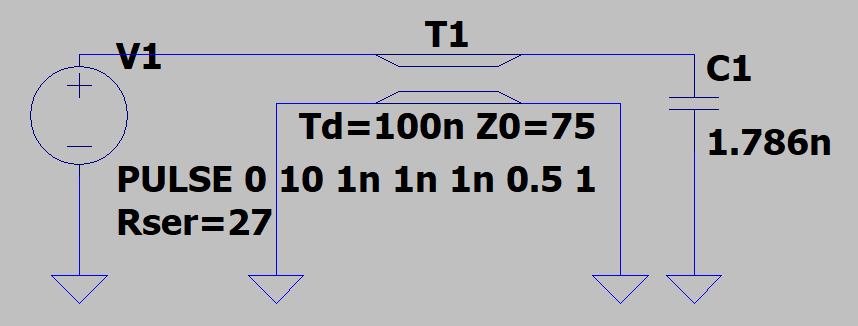
\includegraphics[scale=0.7]{Q1 line.png}\\
    
    \small{Linha simulada através do software LTspice}
\end{center}

Parâmetros:

$C_1 = 1,786$ nF

$u = 2,786\times 10^{8}$ m/s

$l = 27,86$ m


$$V_2(s) = \frac{2E_g}{s} \frac{Z_0}{R_g + Z_0} e^{-Bls} \frac{\frac{1}{sC_1}}{\frac{1}{sC_1}+Z_0} = 2v^+ e^{-Bls} \left[ \frac{1}{s} - \frac{1}{s+\frac{1}{Z_0C_1}}\right], v^+ = \frac{E_g \times Z_0}{R_g + Z_0}, B = \frac{1}{u}$$

$$v_2(t) = v^+ H(t-Bl)\left[ 2 - 2e^{-\frac{(t-Bl)}{\tau}} \right], \tau = Z_0C_1$$

$$v_2^-(t) = v^+ H(t-Bl)\left[ 1 - 2e^{-\frac{(t-Bl)}{\tau}} \right]$$

$$v_1(t) = v^+ H(t) + v^+ H(t-2Bl)\left[ 1 - 2e^{-\frac{(t-2Bl)}{\tau}} \right](1 + \rho_g), \rho_g = \frac{R_g-Z_0}{R_g+Z_0}$$

$$v_1(t\rightarrow\infty)=v_2(t\rightarrow\infty)=E_g$$


\paragraph{a)}

$v_1(t=0,2^-\mu s) = 7,35294$ V

\ \ $v_1(t=0,2^+\mu s) = 3,46021$ V

\paragraph{b)}

$v_1(t=\infty) = 10$ V

\ \ $v_2(t=\infty) = 10$ V


\paragraph{c) Com os valores para os itens a) e d) apresentados no primeiro gráfico e uma aproximação (1ms$>>$100ns) de b) (t$\rightarrow \infty$) no segundo gráfico.}

\begin{center}
    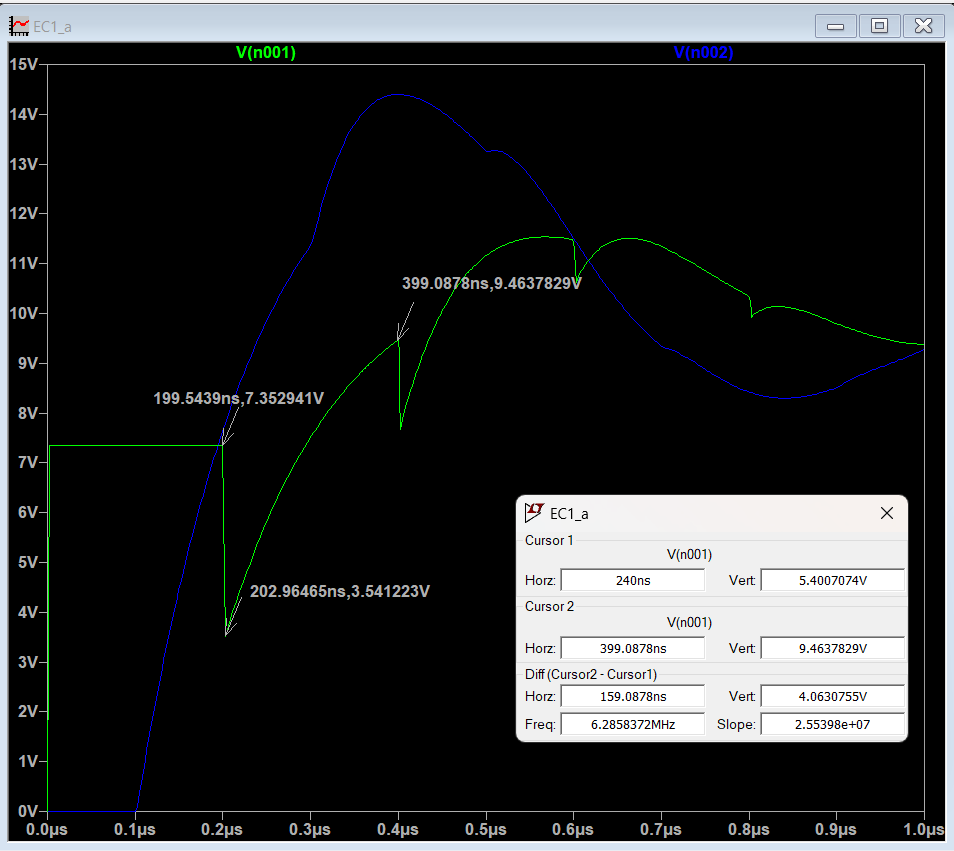
\includegraphics[scale=0.5]{Q1 item c 1.png}\\
    
    \small{Transiente em $0 \le t \le 1\mu s$}\\
    
    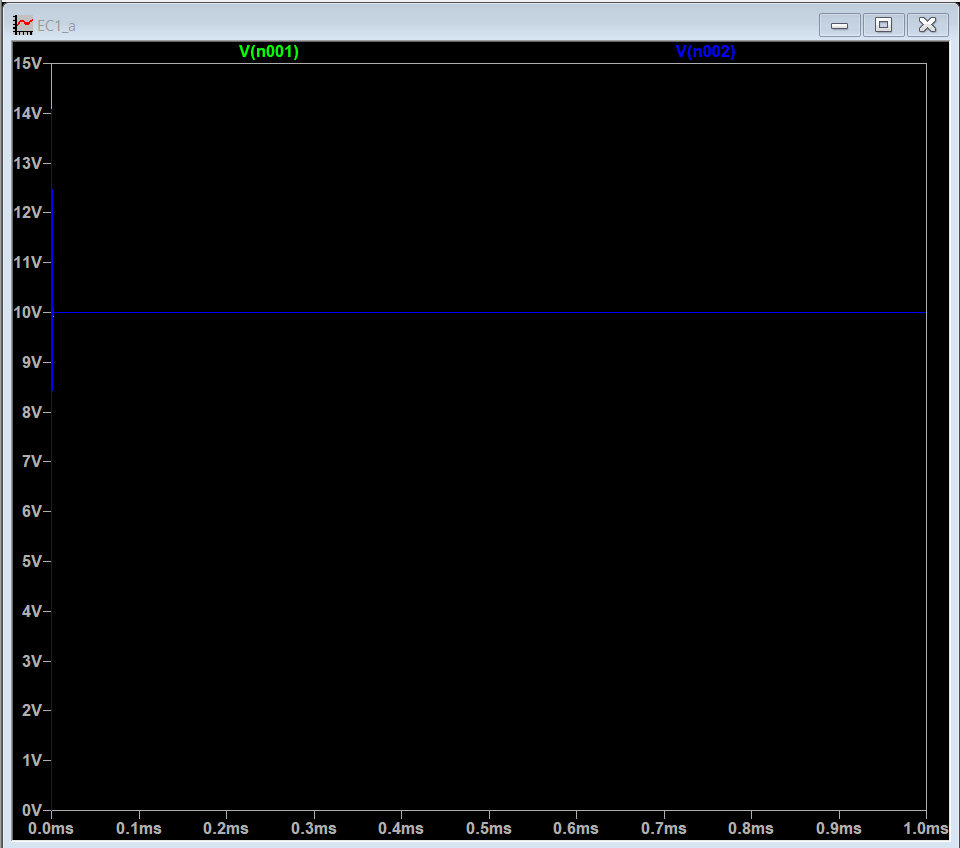
\includegraphics[scale=0.5]{Q1 item c 2.png}\\
    
    \small{Transiente em $0 \le t \le 1ms$}\\
\end{center}

\paragraph{d)}

$\tau = 133,95$ ns

\ \ $v_1(t=0,39999\mu s) = 9,49633$ V

\paragraph{e) Para o caso com perdas mas sem distorção:}
$A = 7,786$ mNp/m
$$L = \frac{Z_0}{u}, C = \frac{1}{Z_0u}$$
$$R = A\times Z_0, G = \frac{A}{Z_0}$$

\ \ $L = 269,20316$ nH/m

\ \ $C = 47,85834$ pF/m

\ \ $R = 0,58395$ $\Omega$/m

\ \ $G = 0,10381$ mS/m

$$v_2(t) = v^+ e^{-Al} H(t-Bl)\left[ 2 - 2e^{-\frac{(t-Bl)}{\tau}} \right]$$

$$v_2^-(t) = v^+ e^{-Al} H(t-Bl)\left[ 1 - 2e^{-\frac{(t-Bl)}{\tau}} \right]$$

$$v_1^-(t) = v^+ e^{-2Al} H(t-2Bl)\left[ 1 - 2e^{-\frac{(t-2Bl)}{\tau}} \right]$$

$$v_1(t) = v^+ H(t) + v^+ e^{-2Al} H(t-2Bl)\left[ 1 - 2e^{-\frac{(t-2Bl)}{\tau}} \right](1 + \rho_g)$$

\ \ $v_1(t=0,2001\mu s) = 4.83414$ V

\ \ $v_2(t=0,29999\mu s) = 9.17822$ V

\begin{center}
    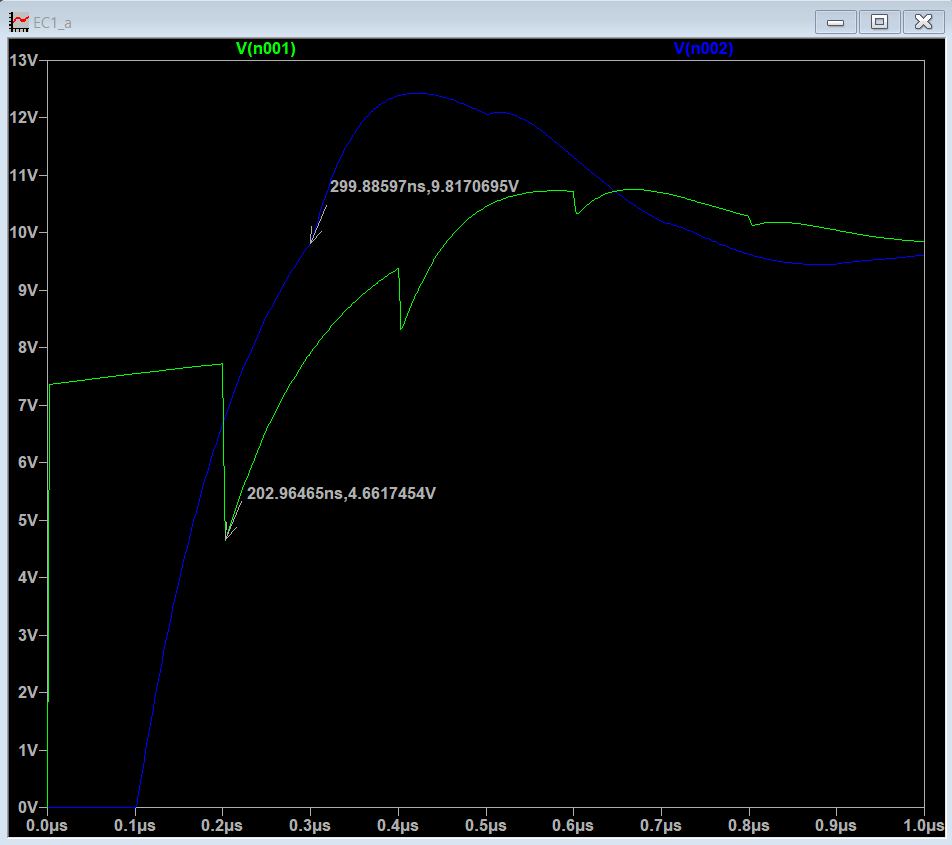
\includegraphics[scale=0.5]{Q1 item e.png}\\
    
    \small{Modelo com perdas, $0 \le t \le 1\mu s$}\\
\end{center}




A fins de comparação (e pelo fato do LTspice não considerar as perdas no dielétrico), as mesmas simulações foram feitas com os softwares Multisim e ADS (Advanced Design System), e seus resultados são apresentados a seguir:

\begin{center}
    \small{\textbf{Modelo no Multisim}}\\

    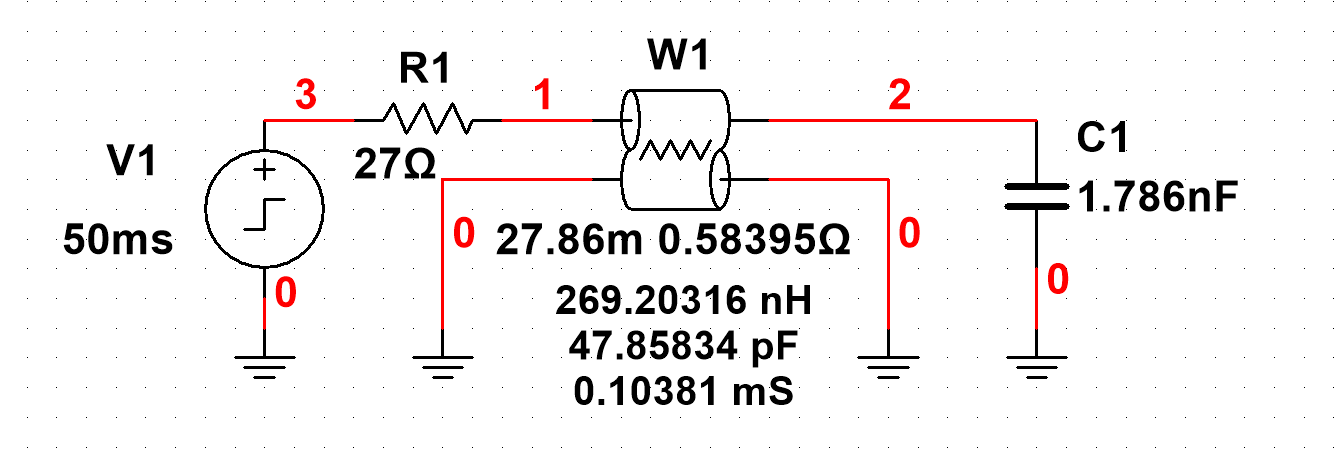
\includegraphics[scale=0.45]{multisim.png}\\
    
    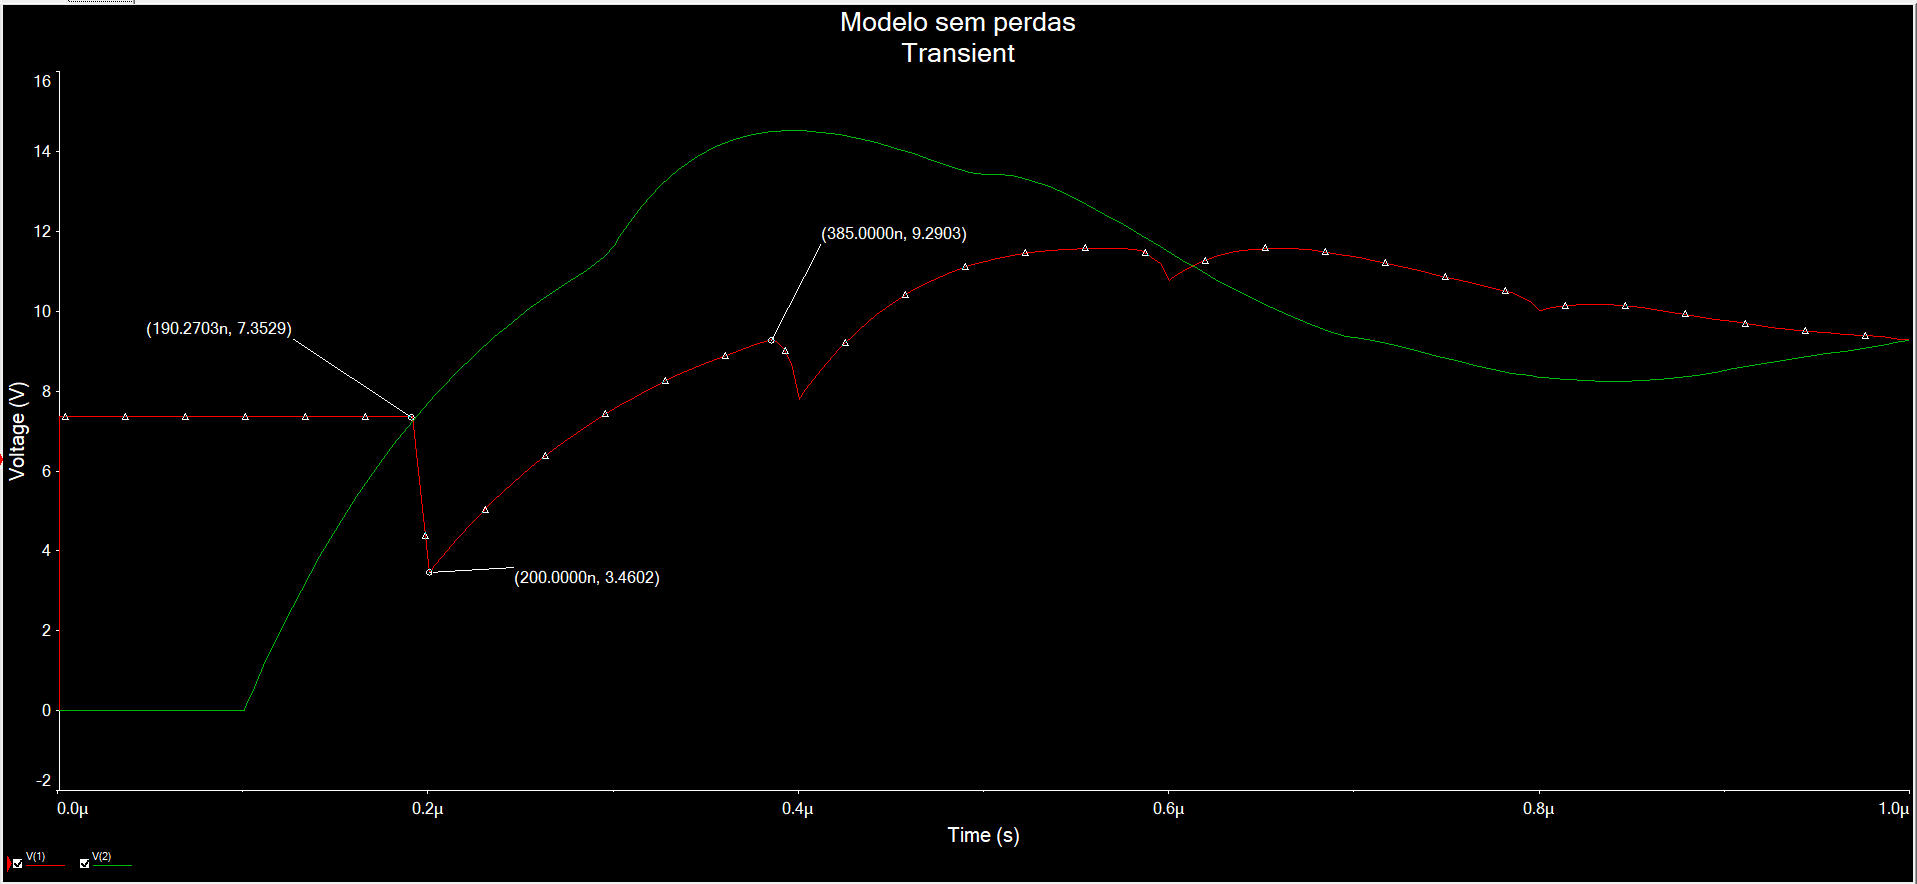
\includegraphics[scale=0.3]{multisim c.png}\\
    
    \small{Modelo sem perdas, transiente em $0 \le t \le 1\mu s$}\\

    
    
    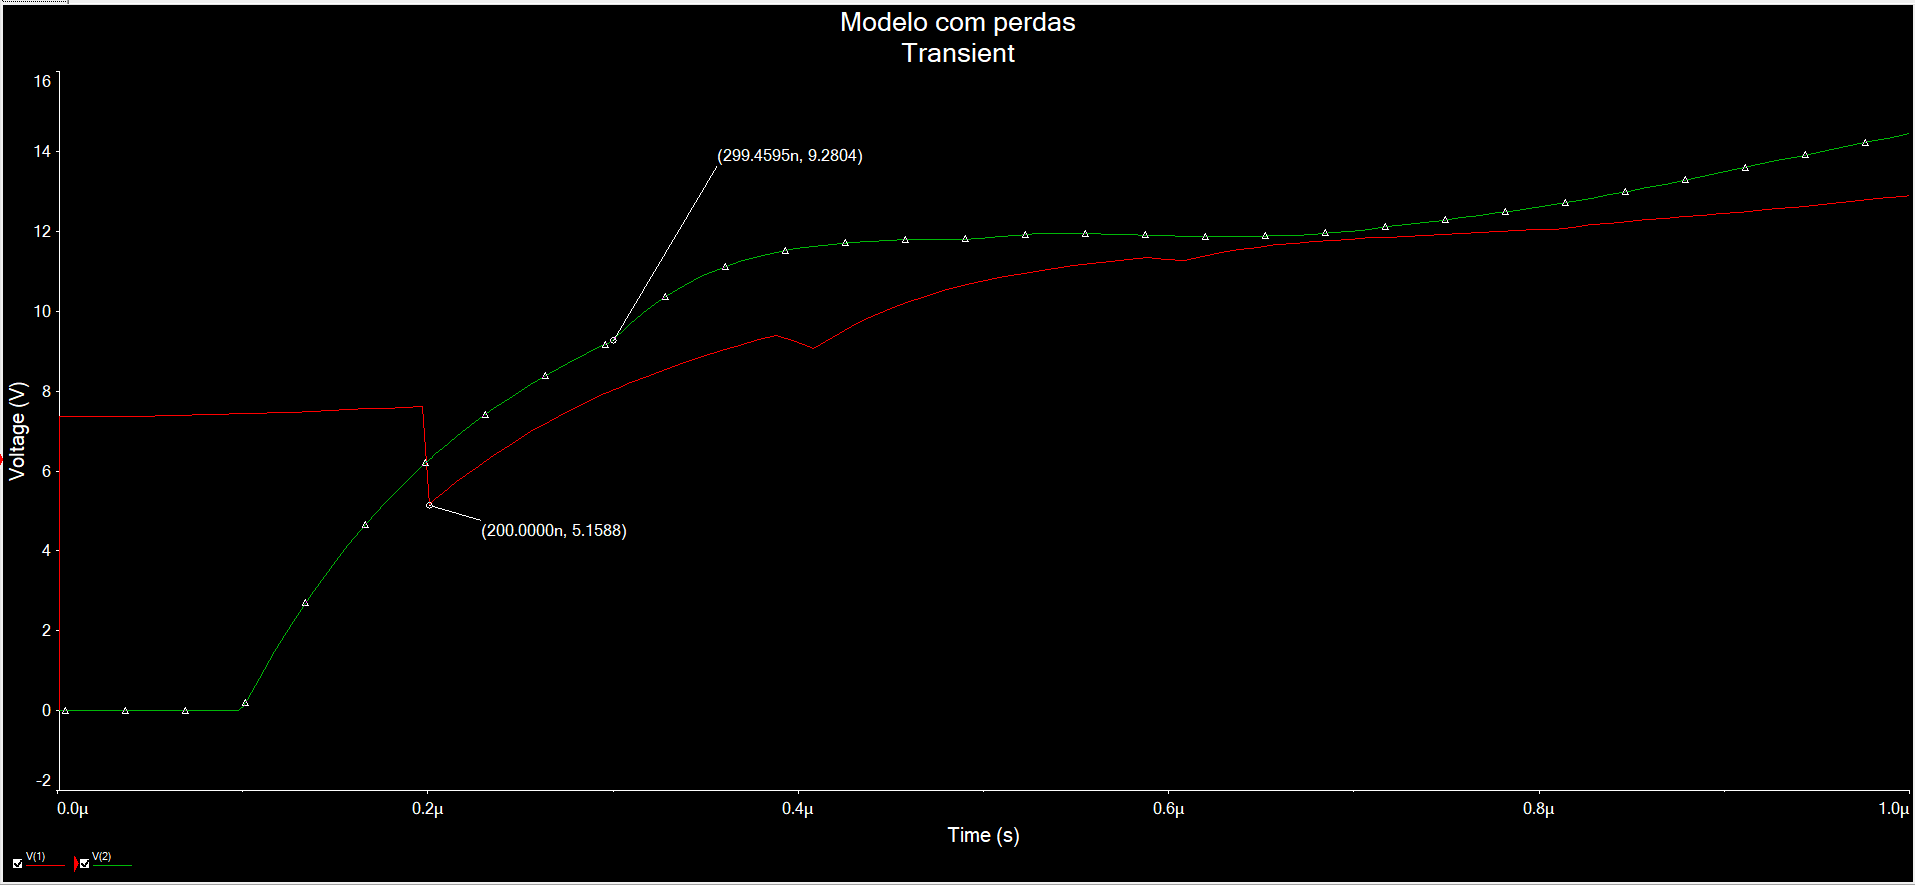
\includegraphics[scale=0.3]{multisim e.png}\\
    
    \small{Modelo com perdas, transiente em $0 \le t \le 1ms$}\\
\end{center}

\begin{center}
    \small{\textbf{Modelo no ADS}}\\

\hspace{-1.5cm}
    \begin{minipage}{0.65\textwidth}
        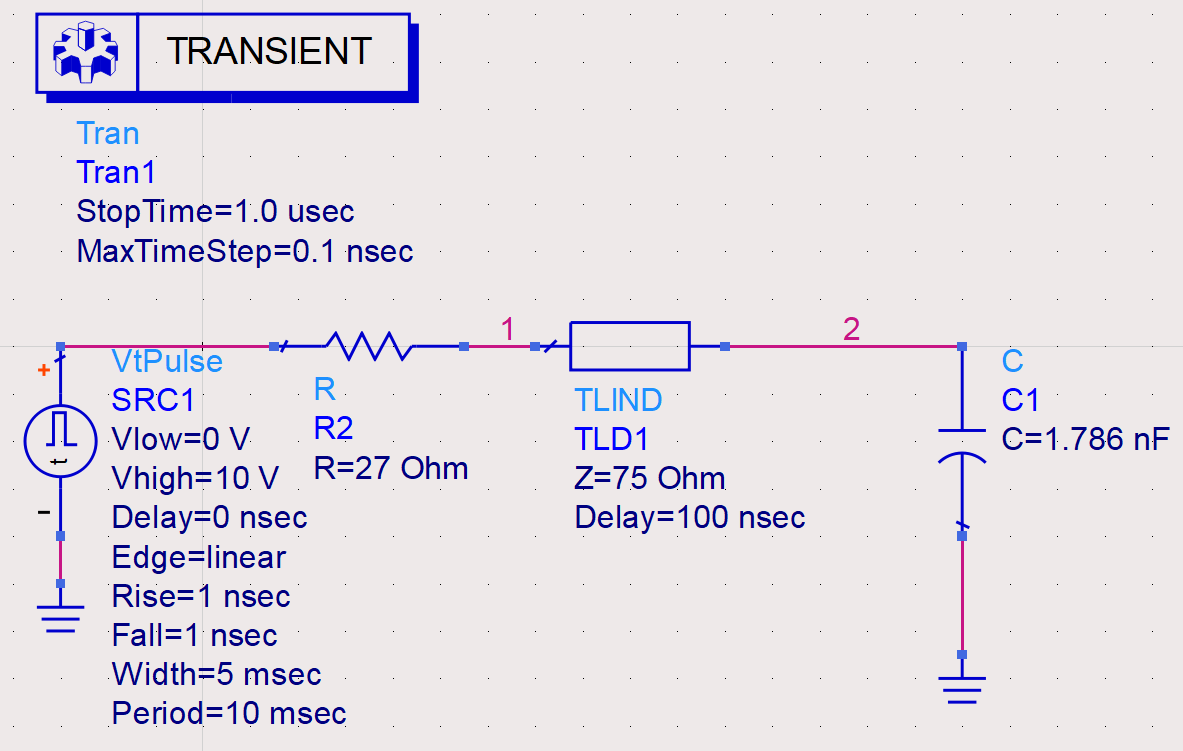
\includegraphics[scale=0.3]{ads1.png}\\
    \end{minipage}
    \begin{minipage}{0.35\textwidth}
        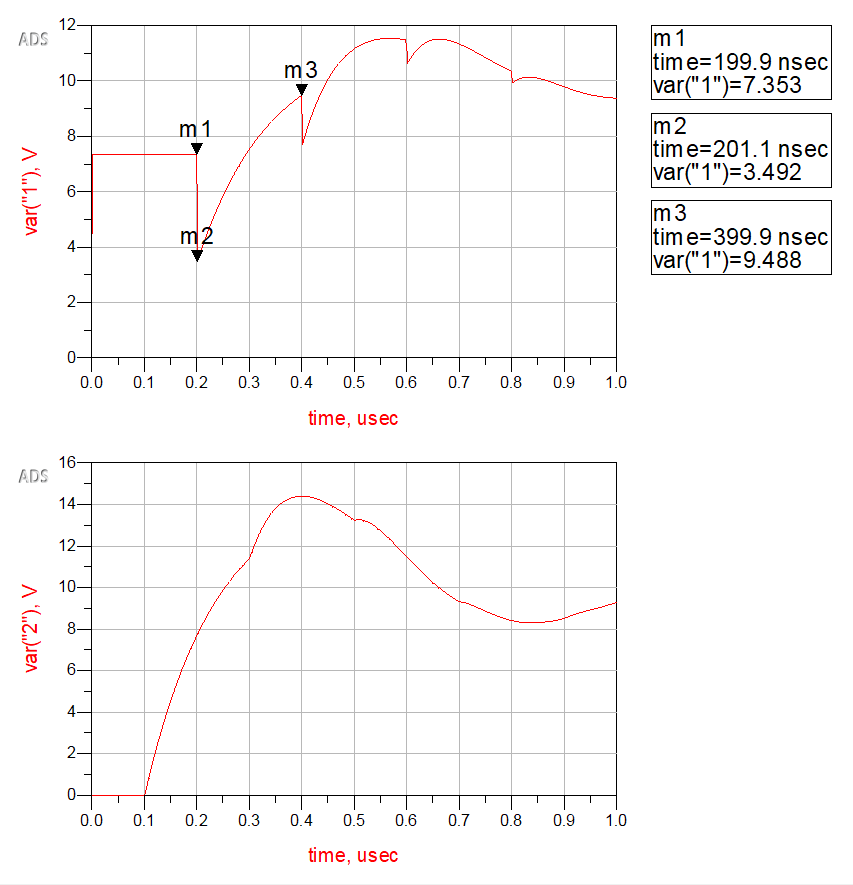
\includegraphics[scale=0.3]{ads2.png}\\
    \end{minipage}

    \small{Modelo sem perdas, transiente em $0 \le t \le 1\mu s$}\\

\break

    \hspace{-1.5cm}
    \begin{minipage}{0.65\textwidth}
        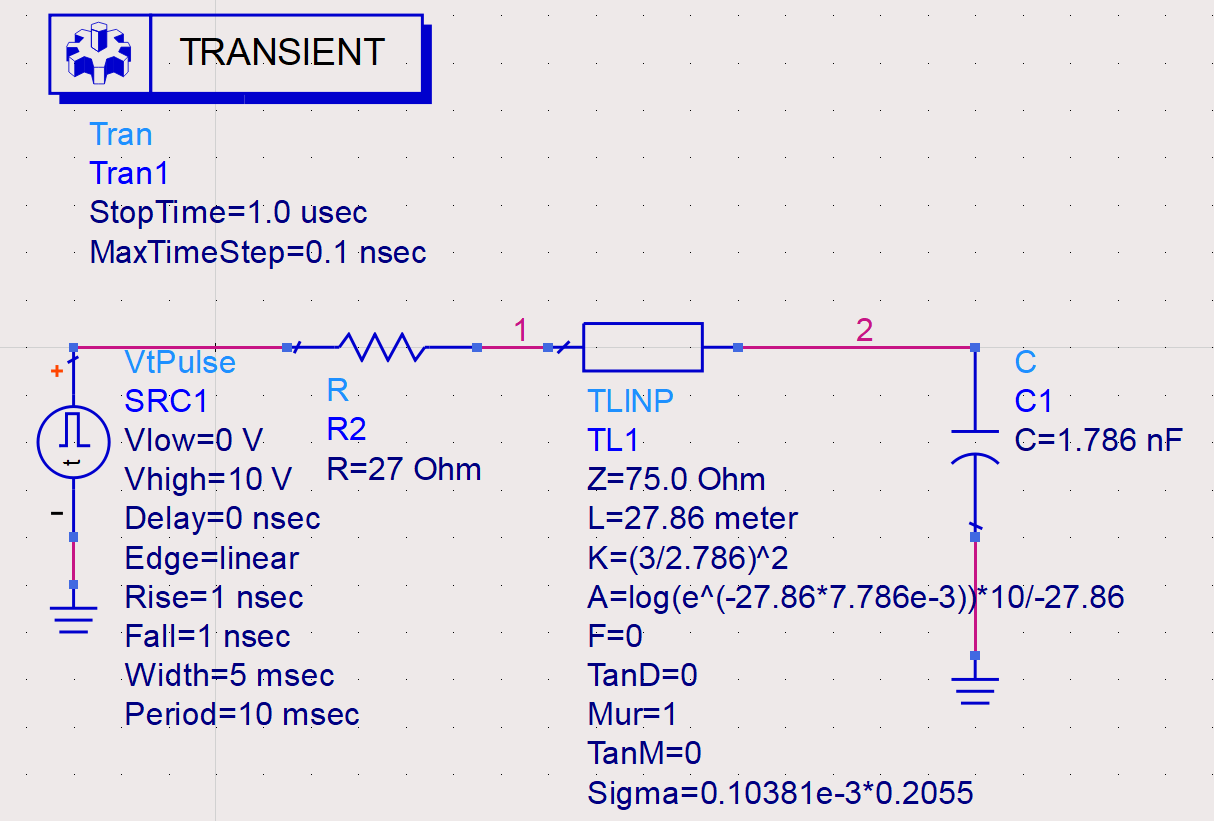
\includegraphics[scale=0.3]{ads3.png}\\
    \end{minipage}
    \begin{minipage}{0.35\textwidth}
        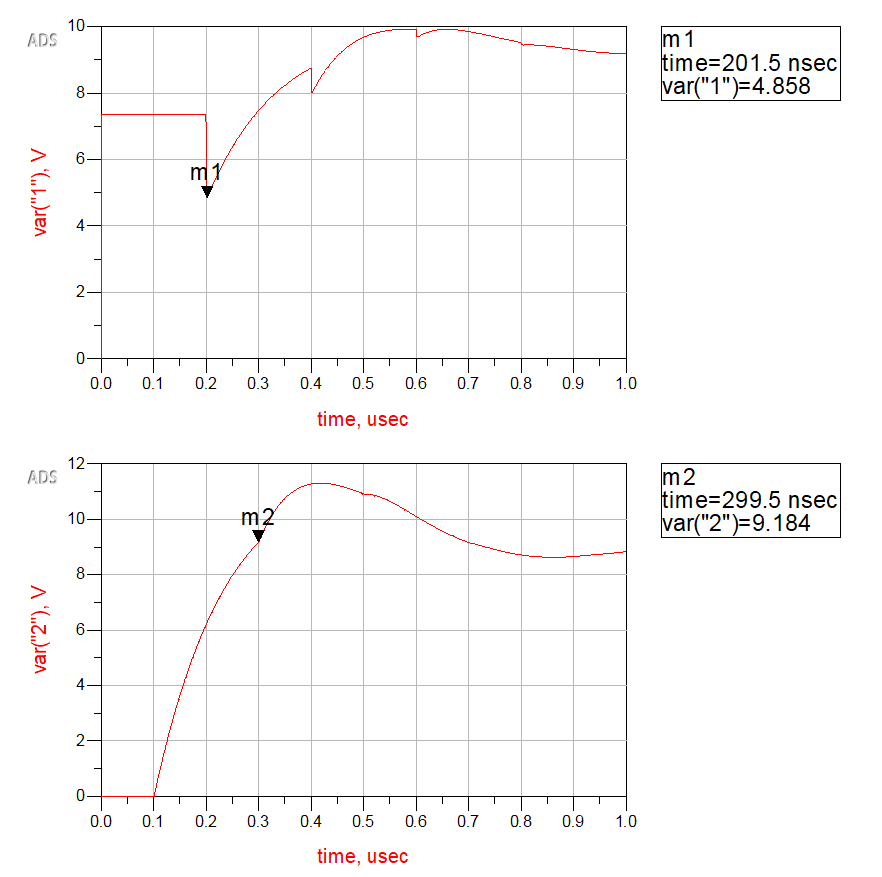
\includegraphics[scale=0.3]{ads4.png}\\
    \end{minipage}

    \small{Modelo com perdas, transiente em $0 \le t \le 1\mu s$}\\

\end{center}


%v_1(t=0,2001\mu s) = 4.83414$ V
%v_2(t=0,29999\mu s) = 9.17822$ V
\hspace{-1.5cm}
    \begin{tabular}{c|c|c|c|c}
         SOFTWARE&$v_1(t=0,2001\mu s)$&Erro relativo (\%) &$v_2(t=0,29999\mu s)$&Erro relativo (\%)\\
         \hline
         LTspice&4,6617454 V& 3,5661896 &9,8170695 V&6,9604945\\
         Multisim&5,1588 V& 6,7159826 &9,2804 V&1,1132878\\
         ADS&4,858 V& 0,4935728 &9,184 V&0,0629752\\
    \end{tabular}
    \begin{center}
        \small{Tabela comparativa entre simuladores para o problema com perdas}
    \end{center}

\newpage
%-------------------------------------------
%-------------------------------------------

\section{}

\paragraph{a) Modelo de linha ideal\\ \\}


    \hspace{-1.5cm} 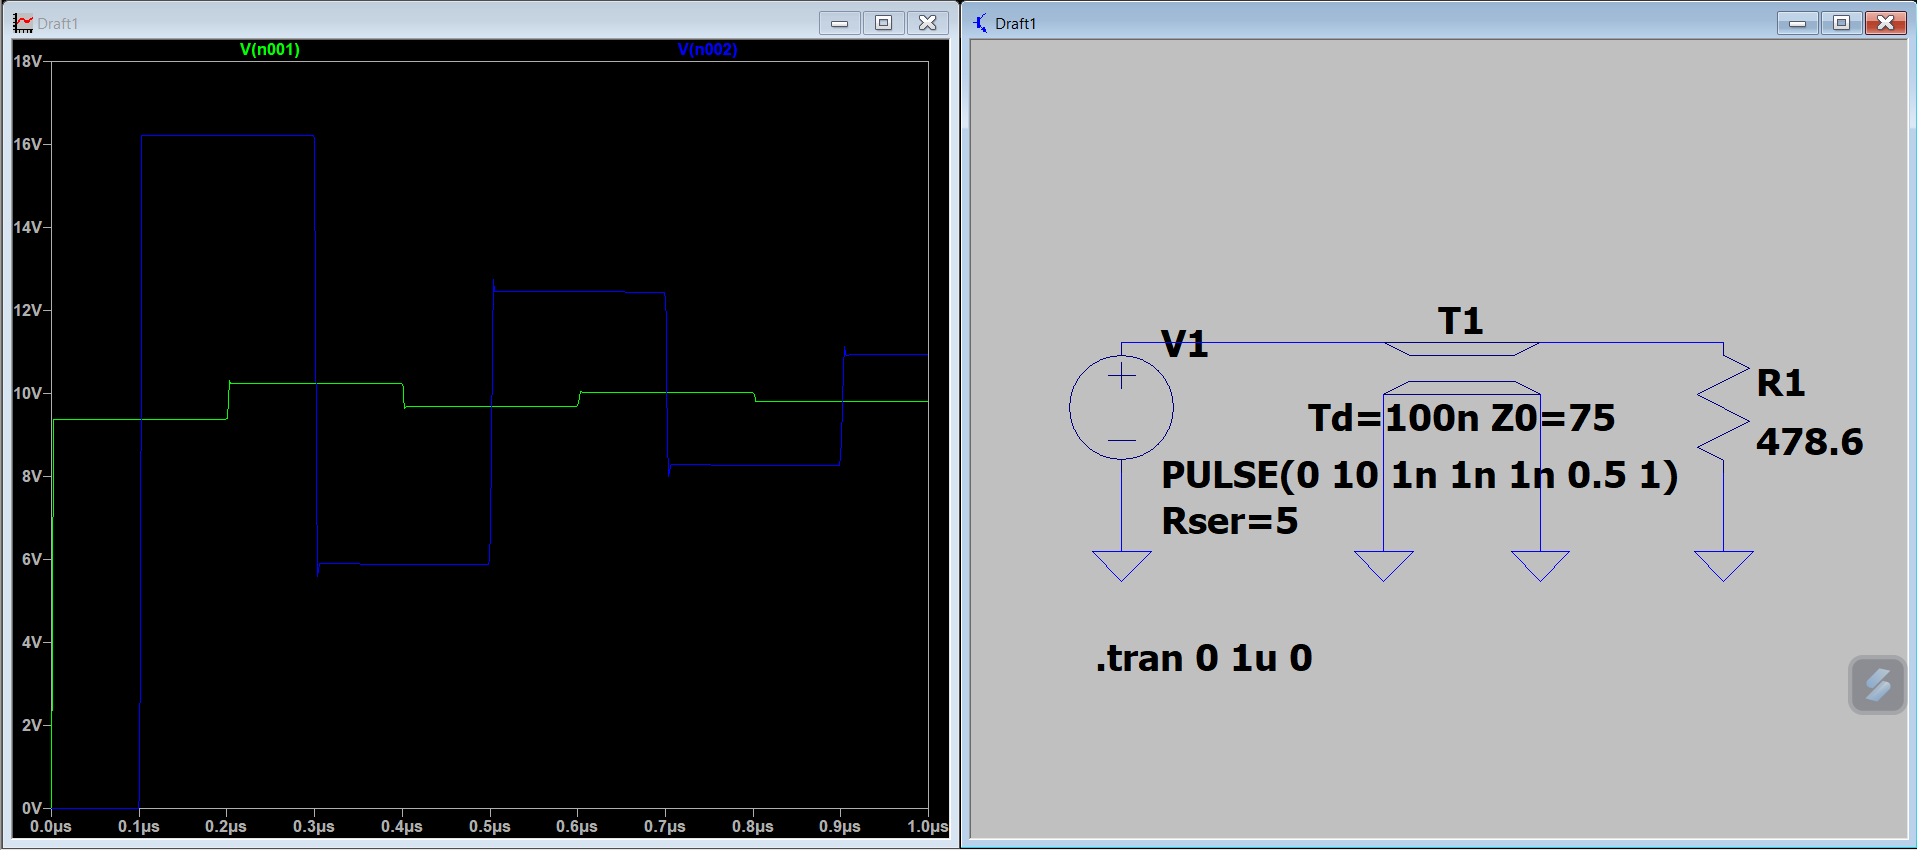
\includegraphics[scale=0.35]{Q2 item a.png}
    \begin{center}
        \small{Linha simulada através do software LTspice}
    \end{center}

\paragraph{b)}

$C_{10}=133,33333$ pF,
$L_{10}=750,0$ nH

\ \ $C_{20}=66,66667$ pF,
$L_{20}=375,0$ nH

    {\centering Modelo com 10 pedaços:\\}

    \hspace{-1.5cm} 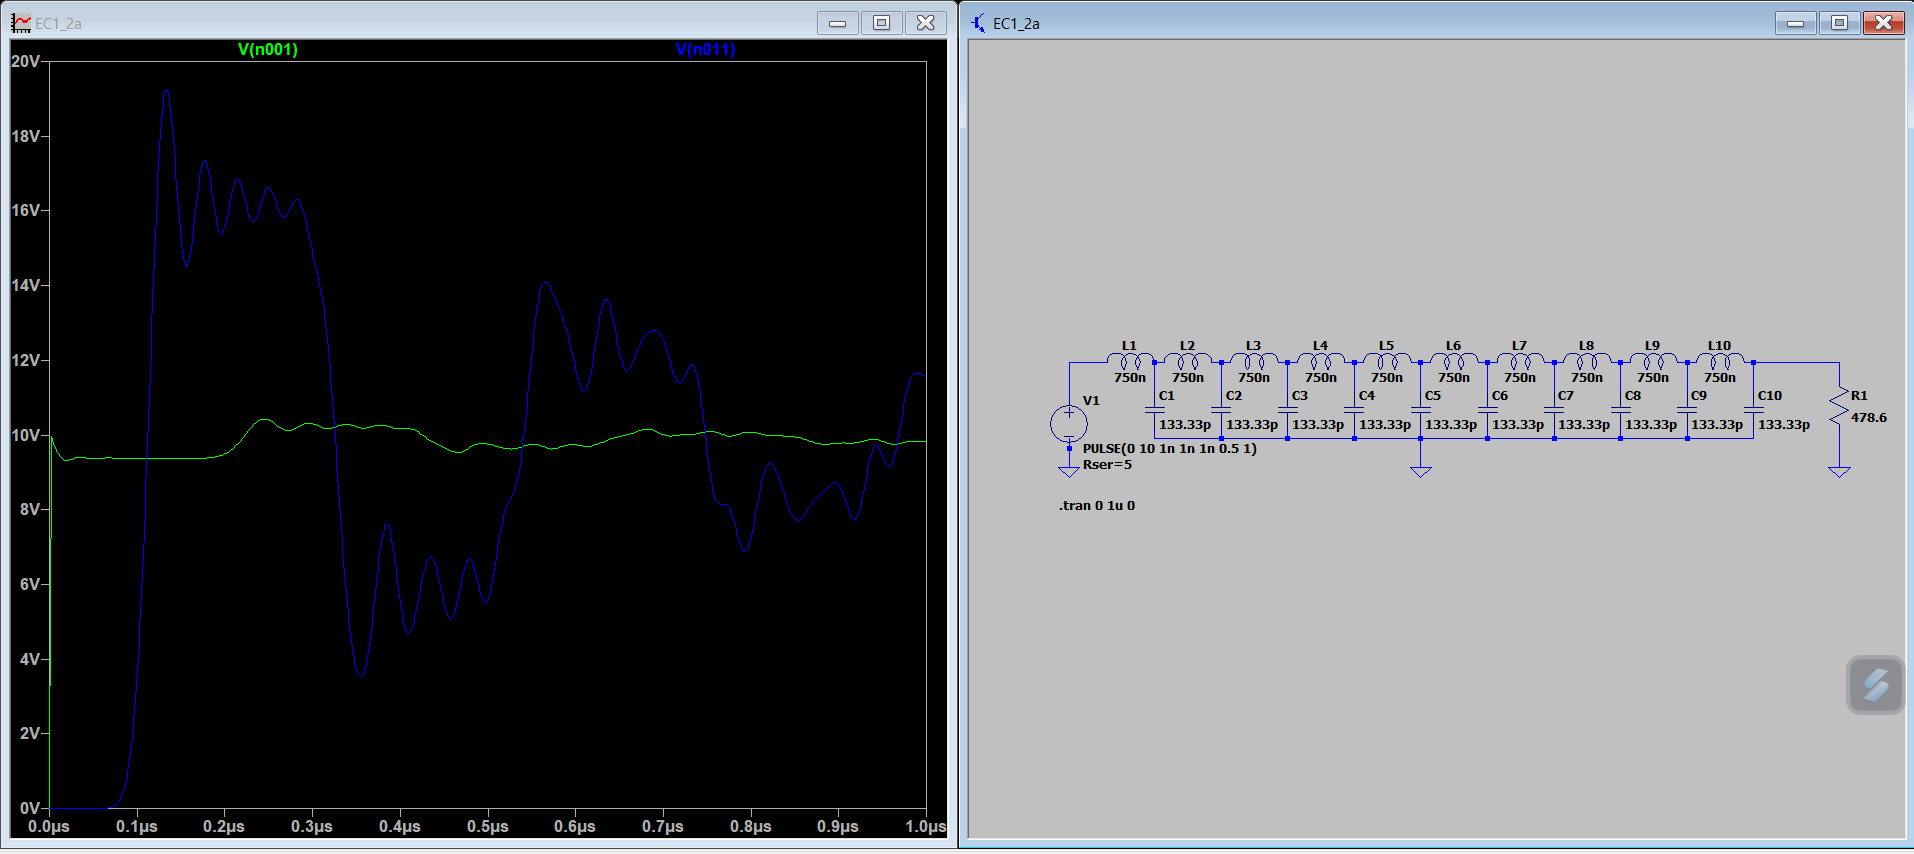
\includegraphics[scale=0.35]{Q2 item b 10.png}

\break

    {\centering Modelo com 20 pedaços:\\}

    \hspace{-1.5cm} 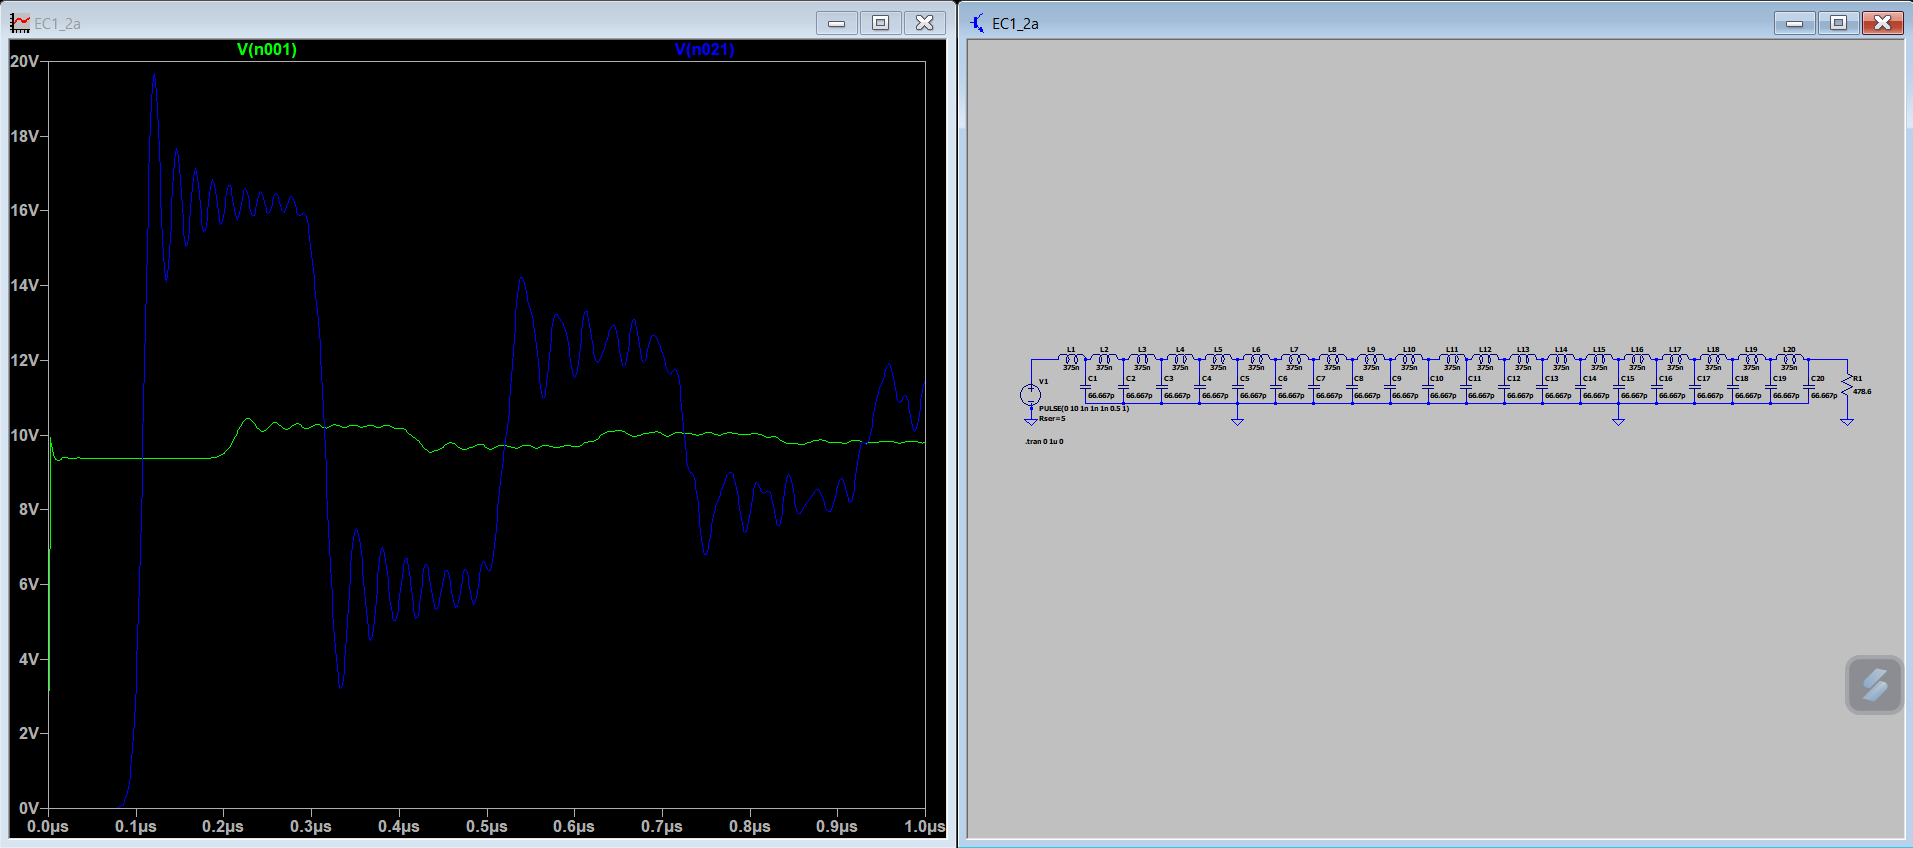
\includegraphics[scale=0.35]{Q2 item b 20.png} \\

Quanto aos valores obtidos, foram calculados com base nas características da linha (indutância e capacitância por metro) e multiplicadas pela parcela da linha para cada caso (para uma linha com \textit{l} metros e \textit{n} pedaços, foi feito o produto com o fator $\Delta z=$ \textit{l/n}).

Os valores das duas simulações parecem tender as amplitudes percebidas no item a), levando em conta a tendência dos respectivos amortecimentos.

Entre os dois modelos, o segundo apresenta uma resposta melhor e mais rápida nos pontos em que ocorre a reflexão (e os valores sofrem trocas abruptas), justamente devido ao fato de sua frequência amortecida ser maior, como esperado do aumento do número de pedaços.

Para valores cada vez maiores espera-se que a resposta se torne mais semelhante a simulação do primeiro item, já que no modelo ideal são idealizados infinitos pedaços.

\end{document}